\chapter{Moduri alternative de funcționare și cazuri speciale}
\label{chap:extra}

 După cum am menționat în \autoref{time}, frecvența citirilor senzorilor de prezență este principalul factor ce limitează numărul de posibilități ale sistemului. În modelul prezentat, fiind o versiune la scară mult redusă, frecvența citirilor aduce două probleme principale:

\begin{enumerate}
\item Obiectele folosite pentru a simula vehiculele devin mult mai scurte;

\item Distanțele mai mici între senzori duc la calcule eronate în cazul obiectelor cu viteze mari. 

\end{enumerate}

 Sistemul real permite scăderea frecvenței citirilor, fară a ieși din limitele performanțelor dorite, în schimbul adăugării unor caracteristici suplimentare.

 \section{Ecran LCD}

\indent \indent Sistemul permite adăugarea unui  \gls{lcd}, ce permite observarea anumitor date intermediare(e.g. viteza unui vehicul în fiecare zonă a sistemului), fară a fi necesară conectarea la computer. Acesta folosește un modul I2C și se conectează la 5V și GND împreună cu restul componentelor, iar adițional, la pinii dedicați SDA și SCL de pe Arduino Mega.

\begin{figure}[!ht]
    \begin{center}
    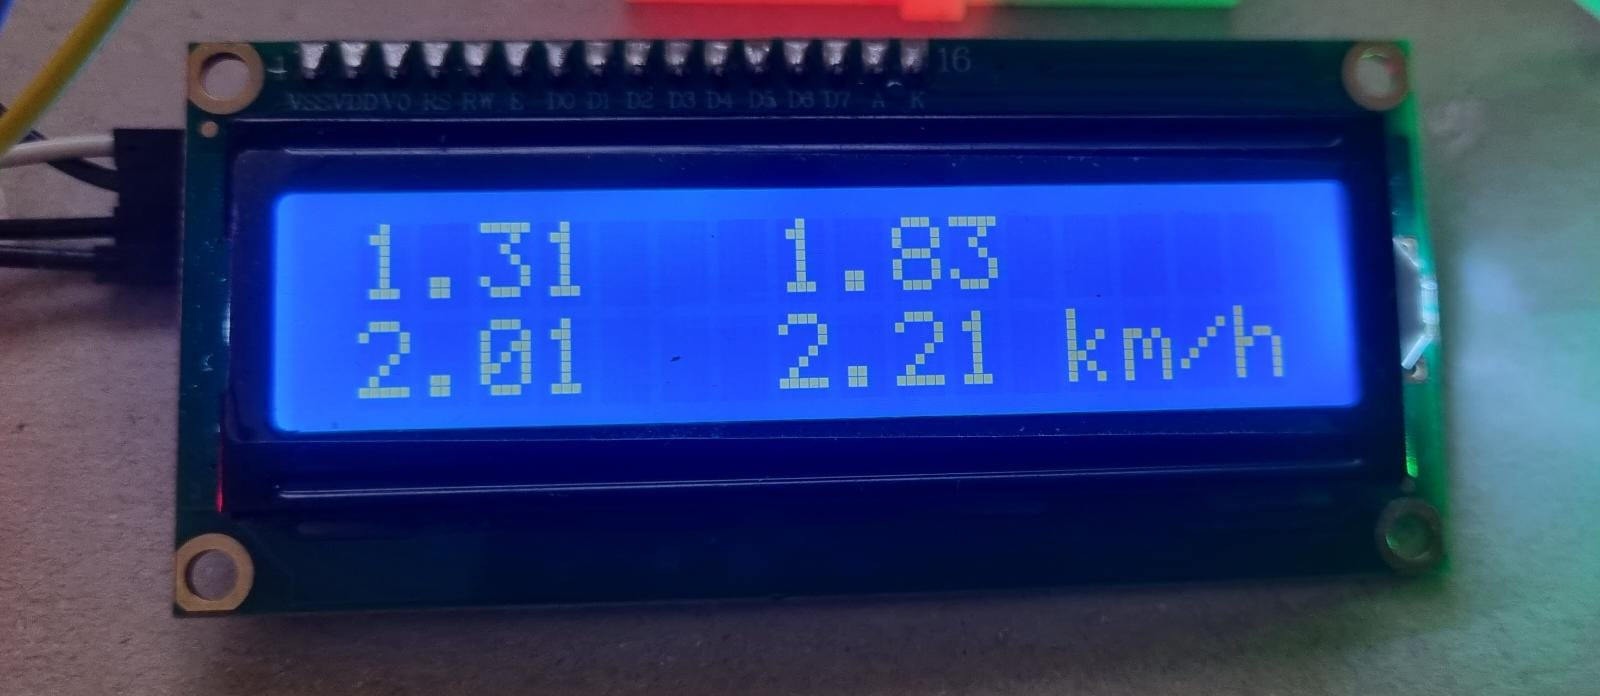
\includegraphics[width=0.5\linewidth,keepaspectratio]{pics/LCD.jpg}
    \end{center}
    \caption{LCD}
    \label{fig:LCD}
\end{figure}


 Pentru utilizarea \gls{lcd}-ului, este nevoie de un task suplimentar (\ref{tlcd}) ce se ocupă cu gestiunea acestuia. Incrementarea semaforului binar SemLCD are loc în TaskProd, la schimbarea oricărei dintre viteze. Acest lucru asigură funcționarea corectă a programului și oprește rescrierea datelor de pe \gls{lcd} la fiecare execuție a task-ului. Astfel, acestea sunt rescrise doar când apare o schimbare. Verificarea și incrementarea valorii variabilei $p$ are loc pentru a asigura faptul că inițializarea display-ului se întâmplă doar la prima rulare a task-ului, ilustrat în \figref{fig:tasklcd}.

  \begin{figure}[!ht]
    \begin{center}
    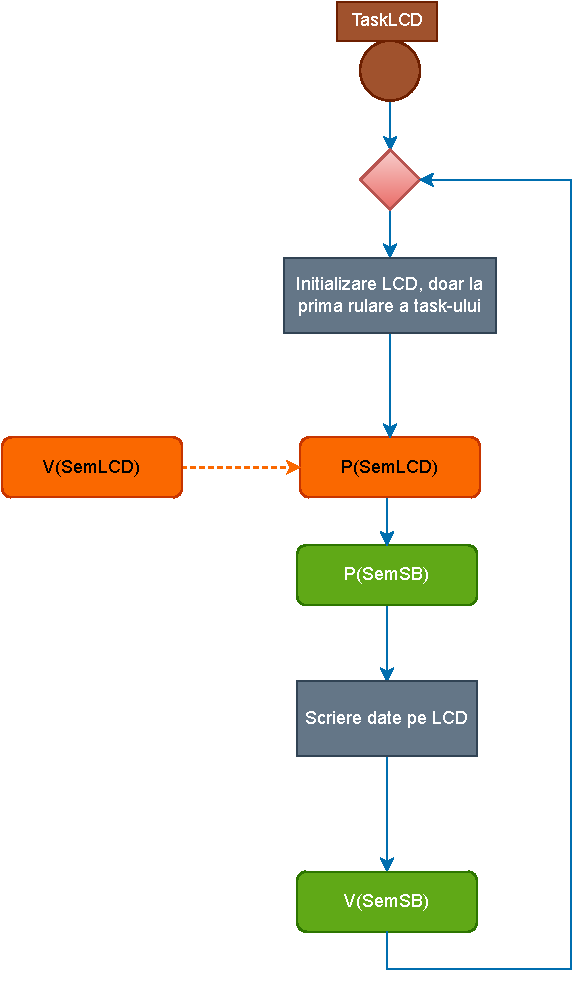
\includegraphics[width=0.6\linewidth,keepaspectratio]{pics/TaskLCD.drawio.pdf}
    \end{center}
    \caption{TaskLCD}
    \label{fig:tasklcd}
\end{figure}

Prezența și funcționarea acestuia necesită sincronizări adiționale între task-uri și un mic delay adăugat la citirile senzorilor. La încercarea rulării în starea inițială, simpla scriere pe LCD bloca tot programul. În cazul soluției găsite de mine pentru rezolvarea problemei, intervalul de timp dintre două citiri a ajuns să fie aproximativ dublu, în jur de 33-34ms.

\section{Citire pe porțiuni a senzorilor} \label{part}

O versiune alternativă a aplicației pentru sistemul de iluminat în timp real este cea în care fiecare senzor este citit individual, într-o rulare a task-ului TaskPROD, iar în TaskCONS se calculează doar o singură viteză, cu ajutorul valorii de timp primite la momentul actual și cea de la execuția anterioară a task-ului. Această metodă este ușor de generalizat. Modificările necesare pentru extinderea sistemului constau în schimbarea dimensiunii buffer-ului din zona comună de date și a transformării semafoarelor binare SemPLIN și SemGOL din \figref{fig:diag_task-uri} în semafoare generalizate. Atât dimensiunea vectorului de date, cât și a semafoarelor va deveni egală cu numărul nou de senzori de prezență \cite{patr}.

În schimb, aici se întâlnește problema scăderii frecvenței citirilor. La citirea unui singur senzor la fiecare rulare a lui TaskCONS, intervalul de timp dintre două citiri ale aceluiași senzor se multiplică cu $n$, unde $n$ este egal cu numărul senzorilor de prezență. Astfel, citirile se realizează la fiecare aproximativ 85ms, în loc de cele 17ms necesare inițial. Acest lucru nu numai că face viteza necesară pentru ca un vehicul să treacă neobservat de $n$ ori mai mică decât cea calculată în \autoref{time}, dar duce și la calcularea greșită a vitezei vehiculului.

În \figref{fig:speed} este reprezentat un exemplu de calcul al vitezei cu citirile aceluiași senzor la un interval de 85 ms, după cum arată variația variabilei t. În acest caz, este calculată viteza $\mathbf{v[0]}$, iar distanța dintre 2 senzori este destul de mică(20cm) pentru a se obține valori foarte mici pentru $t$(variabilă scalară pentru modalitatea de implementare din această secțiune). Viteza se calculează prin împărțire la $t$, ceea ce înseamnă că diferențele mari între valorile sale, relativ la el însuși, duc la obținerea unui rezultat ce nu reflectă realitatea. În exemplul prezentat, asta înseamnă că $\mathbf{v[0]}$ va fi afișat ca 42.35 km/h pentru orice viteză mai mare sau egală cu acest număr, 7.06km/h pentru orice valoare din intervalul [7.06, 42.35) ș.a.m.d.

  \begin{figure}[!ht]
    \begin{center}
    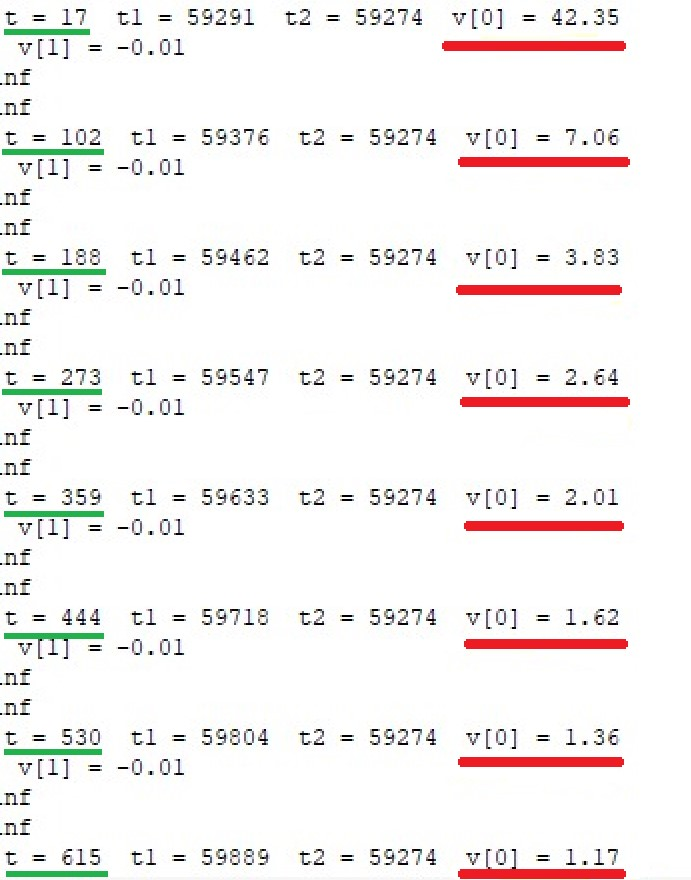
\includegraphics[width=0.585\linewidth,keepaspectratio]{pics/speed.jpg}
    \end{center}
    \caption{Calcul eronat al vitezei}
    \label{fig:speed}
\end{figure}


\subsection{Analiză rezultate} \label{fail}

Rezultatele de pe Serial Monitor, din \figref{fig:speed} pot fi observate și în \figref{fig:v1}, sub formă de grafic. 

\begin{figure}[!ht]
    \begin{center}
    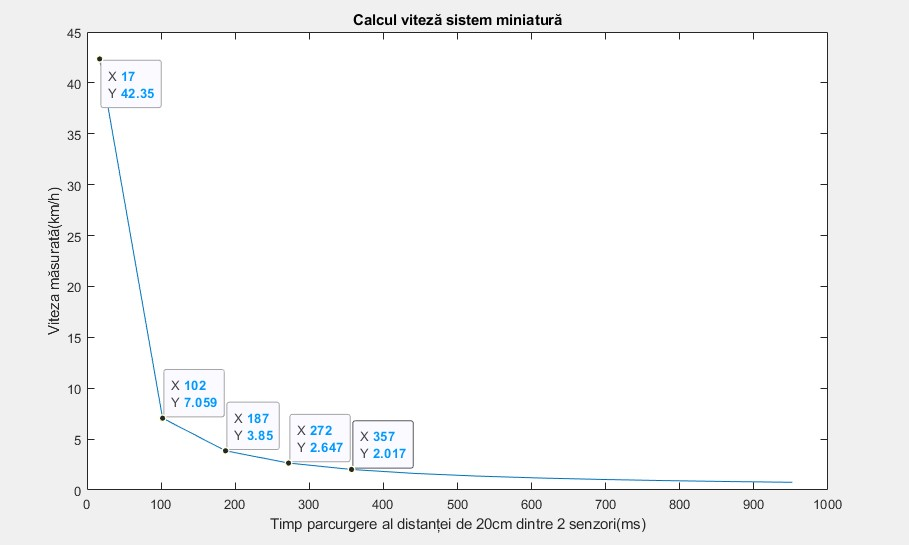
\includegraphics[width=0.9\linewidth,keepaspectratio]{pics/v1.jpg}
    \end{center}
    \caption{Comportarea sistemului mod 1: distanța între senzori 20 cm}
    \label{fig:v1}
\end{figure}

În \figref{fig:v2} am realizat același calcul al vitezei, la modificarea distanței dintre senzori la 35m, în concordanță cu sistemul real. Forma graficului rămâne aceeași, iar singura diferență este creșterea valorii vitezei, direct proporțional cu distanța. 

\begin{figure}[!ht]
    \begin{center}
    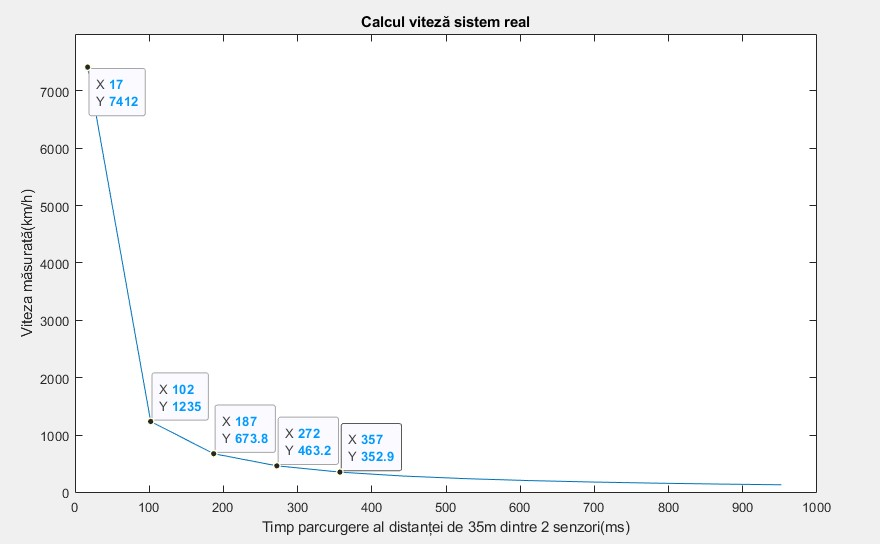
\includegraphics[width=0.9\linewidth,keepaspectratio]{pics/v2.jpg}
    \end{center}
    \caption{Comportarea sistemului mod 2: distanța între senzori 35 m}
    \label{fig:v2}
\end{figure}

În schimb, dacă extind graficul până la momentele de timp în care viteza ar avea valori mai realiste pentru un automobil, ca în \figref{fig:vmare} și \figref{fig:vmic}, se poate observa cum eroarea maximă posibilă, egală cu diferența între două viteze consecutive de pe grafic, începe să scadă. 

\begin{figure}[!ht]
    \begin{center}
    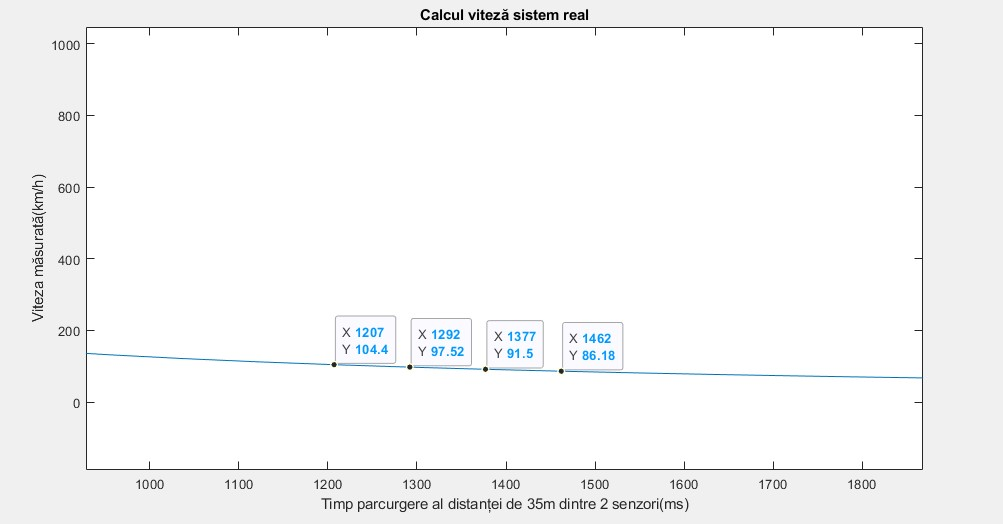
\includegraphics[scale = 0.5]{pics/vmare.jpg}
    \end{center}
    \caption{Eroare posibilă la viteze mari}
    \label{fig:vmare}
\end{figure}

\begin{figure}[!ht]
    \begin{center}
    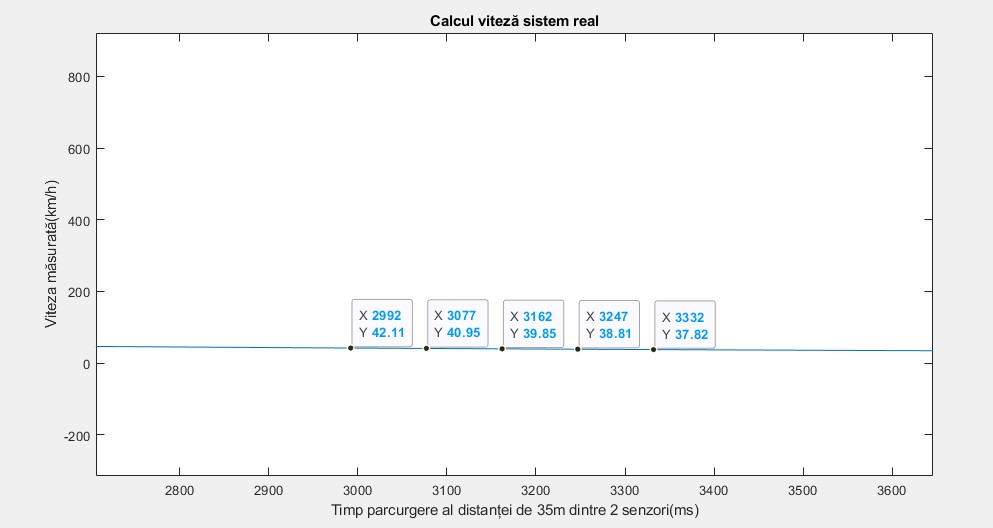
\includegraphics[scale = 0.5]{pics/vmic.jpg}
    \end{center}
    \caption{Eroare posibilă la viteze mici}
    \label{fig:vmic}
\end{figure}

În concluzie, eroarea maximă posibilă pentru măsurarea vitezei devine din ce în ce mai mică, la scăderea vitezei obiectului observat, iar acest proces poate fi grăbit prin mărirea distanței dintre senzori. Astfel, aceste valori pot fi ajustate pentru un sistem de iluminare publică, în funcție de intervalul numeric în care poate fi încadrată viteza vehiculelor pe acea porțiune de drum.

\section{Colectare date valori viteză} \label{collect}

Din moment ce sistemul, în starea sa de bază, deja calculează vitezele vehiculelor pe fiecare porțiune de drum, nu este dificilă modificarea acestuia pentru a salva într-o variabilă vectorială numărul automobilelor ce depășesc o anumită viteză în porțiunea respectivă. Deși am stabilit în \autoref{part} faptul că viteza măsurată nu este niciodată exactă cu această metodă, valorile obținute sunt destul de apropiate de cele reale pentru a servi, de exemplu,  autorităților locale. Datele pot fi folosite, împreună cu statisticile avute deja(e.g. locații frecvente ale accidentelor din trafic) la alegerea locațiilor pentru puncte de instalare a camerelor fixe, sau a punctelor mobile de măsurat viteza.

Factorul ce limitează posibilitatea acestui mod de utilizare al sistemului, este faptul că funcționează doar noaptea. Asta înseamnă că achiziția de date nu se poate realiza pe timp de zi. Pentru a face acest lucru posibil, este nevoie modificări aduse sistemului, atât la partea hardware, cât și la cea software. În primul rând, reiese din prezentarea elementelor hardware din \autoref{senzorir} faptul că nu se pot folosi acești senzori de prezență pe timp de zi, fără a obține date eronate. De aceea este necesară folosirea altor modalități de detectare a prezenței, prin senzori care nu sunt influențați de radiații infraroșii. Un exemplu este utilizarea unor senzori ultrasonici \cite{7456689}, care oferă ca ieșire distanța dintre ei și un obiect. Viteza vehiculelor se poate calcula prin analiza variației acestei distanțe, la 2 momente de timp ulterioare activării unuia dintre senzori.

\begin{figure}[!ht]
    \begin{center}
    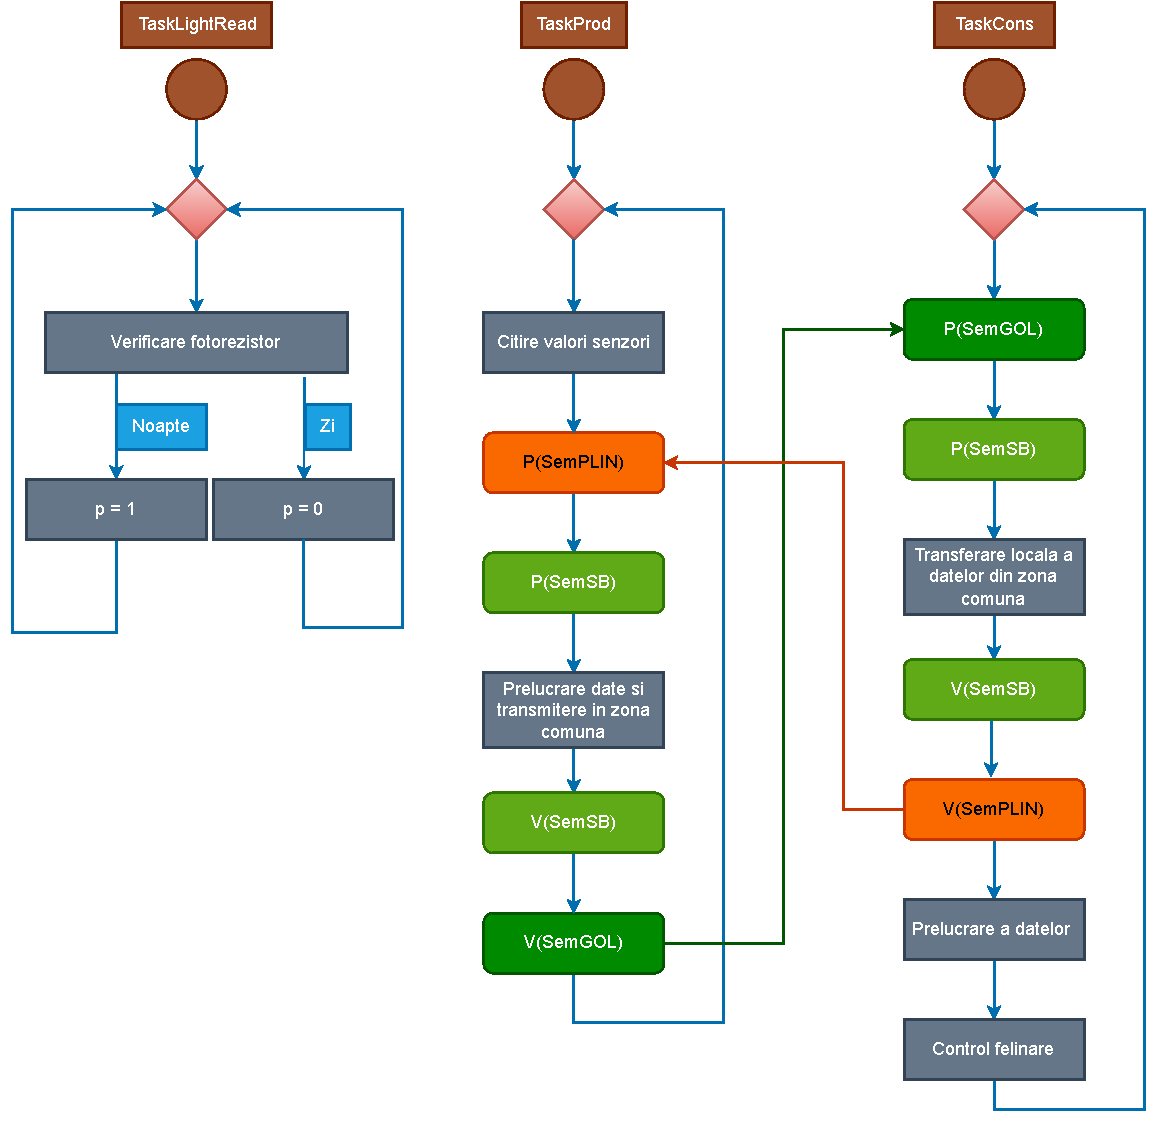
\includegraphics[width=0.9\linewidth,keepaspectratio]{pics/diag2.drawio.pdf}
    \end{center}
    \caption{Diagramă task-uri pentru funcționare pe timp de zi}
    \label{fig:dtask2}
\end{figure}

Pe urmă, trebuie aduse modificări structurii task-urilor, iar acestea sunt ilustrate în \figref{fig:dtask2}. TaskLightRead nu mai reinițializează valorile variabilelor, ci doar modifică valoarea unei variabile $p$. Aceasta îndeplinește rolul de flag, pentru a determina dacă este zi sau noapte. Dacă valoarea sa indică faptul că este zi, partea de \emph{Control felinare} din TaskCons va egala cu 0 valorile din vectorul de luminozitate, pentru stingerea \textbf{completă} a acestora.

\section{Avantaje dublare senzori}
Dublarea senzorilor constă în folosirea a doi senzori de prezență pe porțiunea de drum în care, în mod normal, aș fi folosit unul singur. În funcție de distanța dintre ei și de modul în care sunt utilizate datele citite, aceștia pot îndeplini mai multe scopuri. 

\subsection{Creșterea vitezei maxime la care poate fi detectat un vehicul} \label{speed}
Majoritatea elementelor adiționale adăugate sistemului vor duce la scăderea frecvenței citirii senzorilor de prezență, ceea ce poate cauza trecerea neobservată a vehiculelor, fenomen explicat în \autoref{time}. 

Problema poate fi rezolvată prin înlocuirea fiecărui senzor cu o grupare de doi senzori aflați la distanța $k$ între ei. În această situație, distanța pe care trebuie să o parcurgă un vehicul în intervalul de timp dintre două citiri ale senzorilor, pentru a nu fi detectat, crește cu o valoare egală cu $k$.

În \figref{fig:double} este ilustrat cazul unui vehicul ce nu a fost văzut de primul senzor, dar următoarea citire a avut loc înainte ca acesta să-l depășească și pe al doilea.
\begin{figure}[!ht]
    \begin{center}
    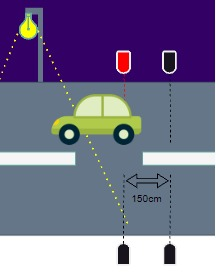
\includegraphics[width=0.3\linewidth,keepaspectratio]{pics/double.jpg}
    \end{center}
    \caption{Creșterea vitezei maxime la care poate fi detectat un vehicul, prin dublarea senzorilor}
    \label{fig:double}
\end{figure}
În acest caz, considerând $k=150$cm și citirea senzorilor la fiecare 85 ms, viteza maximă cu care un vehicul cu lungimea de 190cm poate să se deplaseze fără să fie vreodată neobservat crește de la 80.47 km/h la 144km/h. Counter-ul ce determină aprinderea următorului felinar se va comporta la fel ca în situația activării primului senzor, dar se va stoca într-o variabilă de tip flag care dintre senzori au fost activați, pentru a ajusta distanța folosită la calcularea vitezei.

\subsection{Permiterea funcționării sistemului în ambele sensuri de circulație} \label{rev}
Un alt lucru făcut posibil de dublarea senzorilor este identificarea sensului de deplasare al unui vehicul. În continuare este prezentat cazul unei străzi cu două benzi și sensuri opuse de circulație. În \figref{fig:dep1} este prezentat momentul depășirii unui senzor de un vehicul aflat pe sensul său de circulație, iar \figref{fig:dep2} este reprezentarea aceluiași vehicul în urma trecerii pe contrasens, în cazul unei depășiri. 
\begin{figure}[!ht]
    \begin{center}
    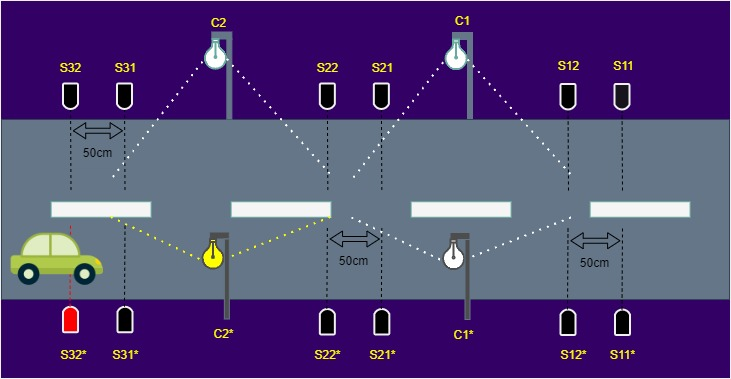
\includegraphics[width=\linewidth,keepaspectratio]{pics/dep1.jpg}
    \end{center}
    \caption{Sistem funcțional pentru ambele sensuri de circulație, moment 1}
    \label{fig:dep1}
\end{figure}

\begin{figure}[!ht]
    \begin{center}
    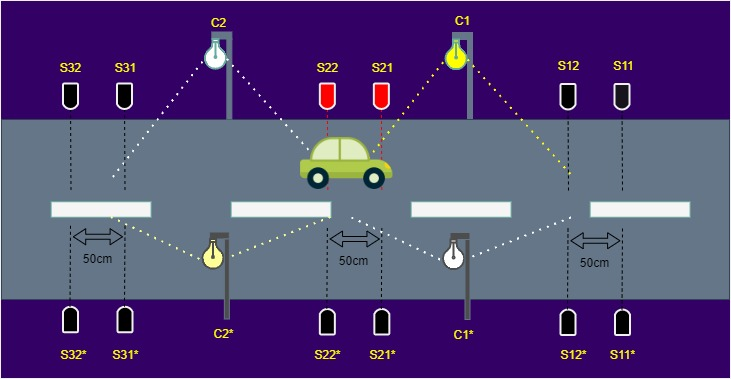
\includegraphics[width=\linewidth,keepaspectratio]{pics/dep2.jpg}
    \end{center}
    \caption{Sistem funcțional pentru ambele sensuri de circulație, moment 2}
    \label{fig:dep2}
\end{figure}

Primul senzor întâlnit în fiecare pereche pe sensul normal ar circulației(S11, S21, S31, S32*, S22*, S12*) este folosit pentru incrementarea sau decrementarea variabilelor counter $\mathbf{c}$ și pentru măsurarea vitezei automobilului, iar valoarea citită de cel de-al doilea(S12, S22, S32, S31*, S21*, S11*) are rolul de a stabili sensul de deplasare. Deoarece înregistrarea momentului de timp la care un vehicul depășește un senzor se face doar la modificarea valorii citită de la acesta (ref), pot verifica tot atunci valoarea citită de la senzorul ajutător. Dacă  aceasta indică prezența unui obiect, înseamnă că vehiculul se află pe contrasens. În această situație, se întâmplă următoarele:

\begin{enumerate}
    \item Se incrementează un element al unui counter $\mathbf{cs}$, corespunzător grupării de senzori (S21-S22).
 \item Se verifică starea counter-ului grupării de senzori anterioare, relativ la sensul de deplasare al vehiculului, pe același sens (în acest caz, S31-S32, și egal cu 0). Dacă aceasta este:
 \begin{itemize}
     \item egală cu 0 - ultimul senzor depășit de vehicul a fost pe cealaltă bandă, deci se decrementează $\mathbf{c}$ pentru cel mai apropiat felinar de pe acea bandă (aici, C2*) 
     \item mai mare ca 0 - ultimul senzor depășit de vehicul a fost pe aceeași bandă deci se decrementează $\mathbf{c}$ pentru cel mai apropiat felinar depășit de acesta (aici, C2).   
 \end{itemize}
 \item Se incrementează elementul counter $\mathbf{c}$ pentru stâlpul următor(C1).
 \item Se decrementează valoarea $\mathbf{cs}$ analizată mai sus în urma calculului vitezei, dacă aceasta este mai mare ca 0.
\end{enumerate}

Este important să fie cunoscut sensul de circulație pe care se află vehiculul la depășirea senzorului anterior până la momentul calcului vitezei, deoarece trecerea pe celălalt sens duce la schimbarea valorii  folosite pentru distanța dintre senzori. Noua distanță \textit{d'} este reprezentată în \figref{fig:dist} și, cunoscând lățimea \textit{w} a drumului, se află prin: 
\be
\label{eq:test}
d'=\sqrt{(w/2)^2+(d+50cm)^2}
\ee
\begin{figure}[!ht]
    \begin{center}
    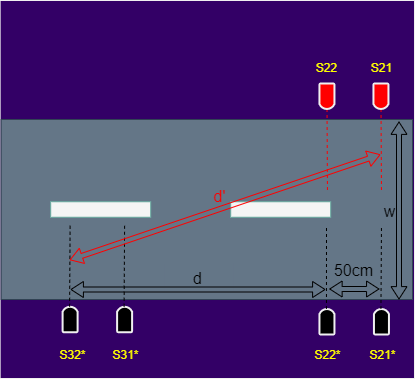
\includegraphics[width=0.4\linewidth,keepaspectratio]{pics/dist.png}
    \end{center}
    \caption{Noua distanță folosită la calcularea vitezei}
    \label{fig:dist}
\end{figure}

O problemă ce trebuie rezolvată pentru implementarea unui astfel de sistem este calculul distanței optime dintre senzorii ce aparțin aceleiași perechi. Aceasta trebuie să fie cât mai mică posibil, pentru a asigura imposibilitatea unui vehicul de a activa doar unul dintre senzori la trecerea pe contrasens. În același timp, ea trebuie să fie și destul de mare pentru ca vehiculul să nu aibă timp să ajungă la al doilea senzor din pereche, înainte să fie detectat de primul, pe sensul normal de mers. În ambele cazuri negative, rezultatul este incrementarea counterului $\mathbf{c}$ al felinarului din spatele vehiculului, în loc de cel din fața sa. Pentru folosirea unei distanțe destul de mici între senzori, este nevoie de o frecvență mare a citirilor, sau de implementarea sistemului pe drumuri cu limite legale mici pentru viteza de circulație.


\section{Soluție implementare sistem pentru cazul unei autostrăzi} \label{hw}

Pentru abordarea cazului implementării sistemului în timp real pe o autostradă cu 4 benzi de circulație(2 pentru fiecare sens, cu separare la mijloc), trebuie rezolvate următoarele probleme:
\begin{itemize}

\item Vitezele mai mari aduc și erori mai mari în măsurarea lor, conform analizei realizate în \autoref{fail}.

\item Vehiculele pot atinge viteze care le permit depășirea neobservată a senzorilor.

\item Variabilele counter din $\mathbf{c}$ pot să primească valori greșite în momentul trecerii a două mașini în paralel.

\item Aprinderea unui singur felinar în fața unui vehicul ce se deplasează cu 130-140 km/h poate fi deranjant pentru ochii șoferului și poate cauza accidente din cauza vizibilității scăzute.
 
\end{itemize}
Soluția propusă de mine constă în câteva modificări aduse sistemului, în starea sa inițială, pentru a rezolva aceste probleme.

În primul rând, toți senzorii de prezență vor fi dublați, pentru creșterea vitezei maxime la care un vehicul poate fi detectat, ca în \autoref{speed}. Apoi, este dublată distanța dintre aceste grupări, pentru a mări precizia cu care este calculată viteza. În  \figref{fig:hw1}, \figref{fig:hw2} și \figref{fig:hw3} sunt surprinse trei momente de interes din trecerea unui vehicul prin sistem. Fiecare senzor din aceste imagini reprezintă, în realitate, câte o pereche de senzori pe care le voi numi, pentru restul secțiunii, grupuri. Pentru a număra corect automobilele din fiecare porțiune a drumului, se folosește câte un grup pentru fiecare bandă de circulație, amândouă influențând valoarea counter-ului $\mathbf{c}$ corespunzător acelorași felinare. Problema vizibilității poate fi rezolvată prin asigurarea faptului că un automobil va avea în orice moment cel puțin două felinare aprinse în fața sa.
\begin{figure}[!ht]
    \begin{center}
    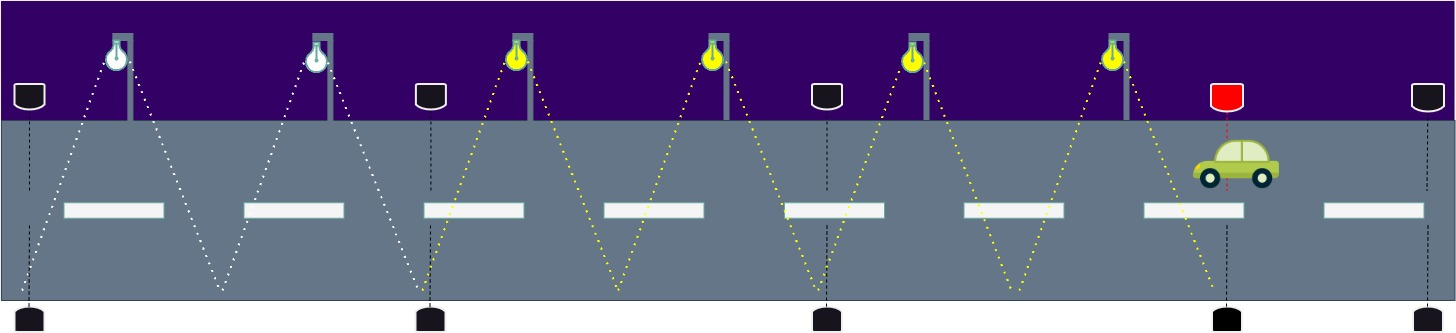
\includegraphics[width=\linewidth,keepaspectratio]{pics/hw1.jpg}
    \end{center}
    \caption{Model sistem autostradă, moment 1}
    \label{fig:hw1}
\end{figure}

\begin{figure}[!ht]
    \begin{center}
    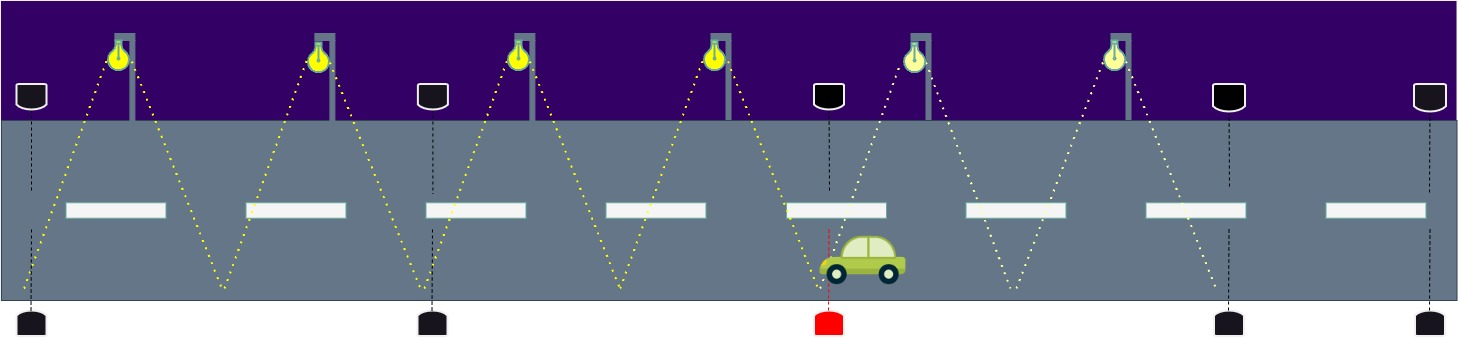
\includegraphics[width=\linewidth,keepaspectratio]{pics/hw2.jpg}
    \end{center}
    \caption{Model sistem autostradă, moment 2}
    \label{fig:hw2}
\end{figure}

\begin{figure}[!ht]
    \begin{center}
    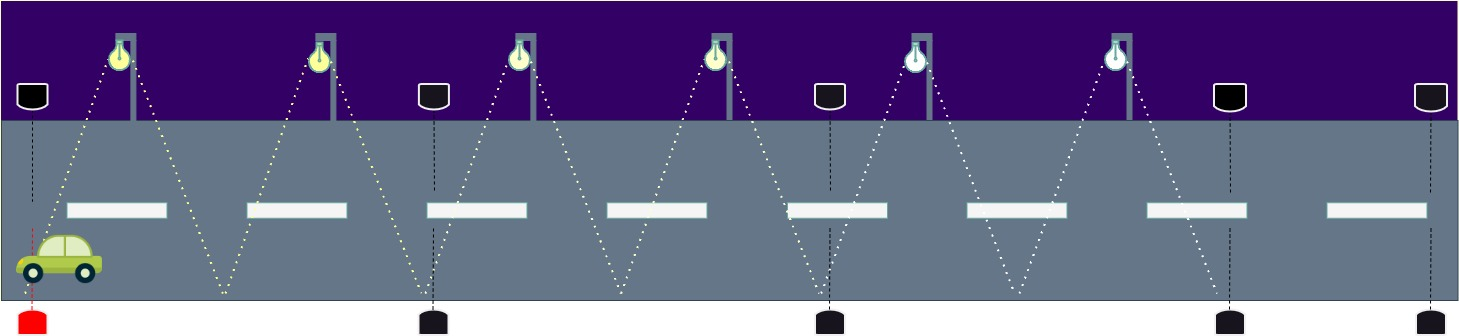
\includegraphics[width=\linewidth,keepaspectratio]{pics/hw3.jpg}
    \end{center}
    \caption{Model sistem autostradă, moment 3}
    \label{fig:hw3}
\end{figure}

 După cum este prezentat în imagini, la momentul depășirii unui grup, cele 2 felinare din urma acestuia se vor stinge, următoarele două vor rămâne aprinse, iar al 3-lea și al 4-lea după acesta se vor aprinde. 
 
 Din moment ce felinarele funcționează în grupuri de câte două, și dimensiunea vectorului $\mathbf{c}$ poate fi înjumătățită. 
 Nu este necesar a fi luat în calcul cazul circulației în sens opus, deoarece pe fiecare bandă a autostrăzii sensul este unic. Astfel, o versiune identică a sistemului poate fi instalată și pentru celelalte două benzi.

